\chapter{Background: Algebraic logic}\label{chap:background3}

\section{Paul Halmos' algebraic logic}

The essence of Halmos' approach to algebraic logic may be explained by this diagram:
\begin{equation}
\vcenter{\hbox{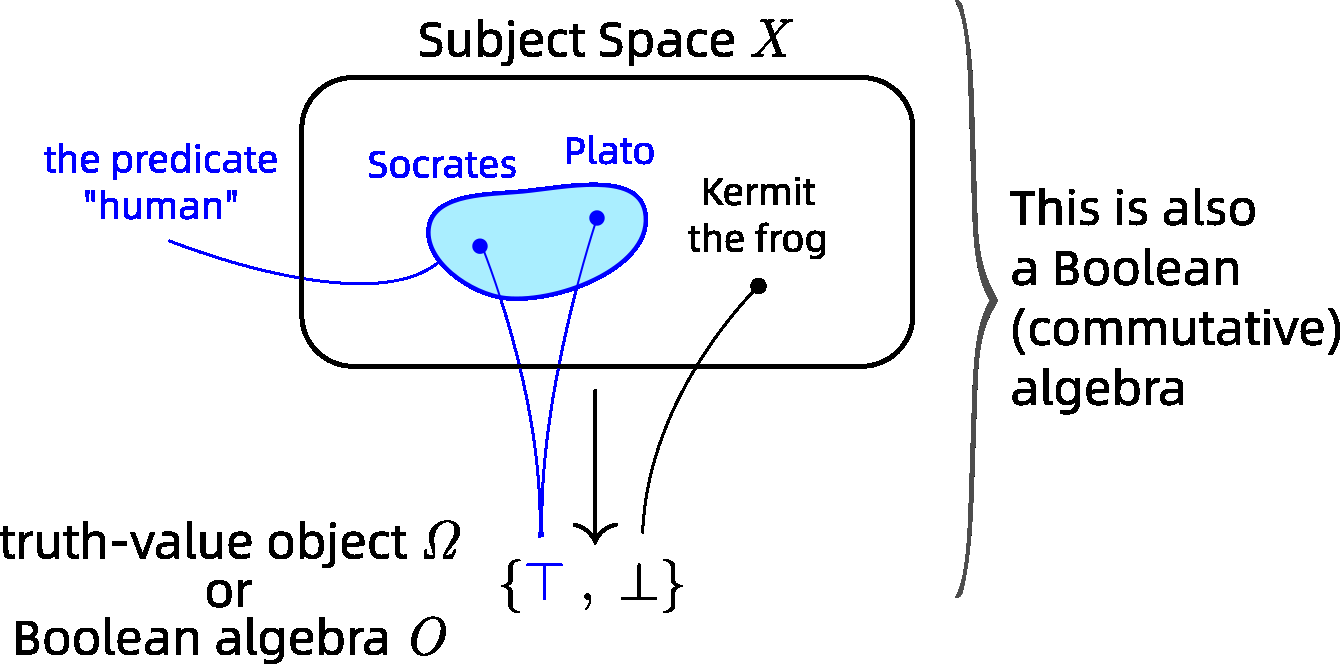
\includegraphics[scale=0.6]{Halmos-nutshell.png}}}
\end{equation}
I coined the term ``Subject Space'' to refer to the space of \textbf{subjects} referred to by predicates.  For example the predicate $\logic{mortal}(\_)$ applies to subjects such as $\logic{Socrates}$ and $\logic{Plato}$ but does not apply to the subject $\logic{Zeus}$.

We all know that propositional logic is isomorphic to the Boolean algebra of sets (Stone's duality theorem).  This is the basis of treating logic as algebra.  But the most sticky point of algebraizing a logic is the treatment of \textbf{predicates}.  Halmos observed that one can form \textbf{propositional functions} from a Subject Space $X$ to a Boolean algebra, and the resulting set of functions would still be a Boolean algebra.  In the above diagram we can see a function mapping subjects to the set $\{ \top, \bot \}$ which is the minimal Boolean algebra $O$, containing only 2 elements, true and false.

The target domain can be a more complex Boolean algebra, as in $X \rightarrow A$.  For example, if Achilles was Zeus's son, he would also be immortal.  So in the proposition space $A$, there would be an implication arrow $\logic{immortal}(\logic{Zeus}) \rightarrow \logic{immortal}(\logic{Achilles})$.  Note that the space $A$ contains points which are just propositions, we cannot access their internal structure.  Anyway, I find that $O = \{ \top, \bot \}$ suffices for our purposes, and we don't need the richer structure of $A$.

More technically, we have the following duality.  Every Boolean algebra $\mathbb{A}$ is isomorphic to the set of all continuous functions from $X$ into $\mathbb{O}$, where $X$ is the dual space of the algebra $\mathbb{A}$, and $\mathbb{O}$ is the Boolean algebra with 2 elements.  If there is a homomorphism $f$ between Boolean algebras $\mathbb{A} \rightarrow \mathbb{B}$ then there is a dual morphism $f^*$ between their dual spaces $Y \rightarrow X$:
\begin{equation}
\begin{tikzcd}[column sep=3cm, row sep=0.6cm]
\mathbb{A} \arrow[r,"f"] \arrow[d,shift left=2,phantom,"\cong"{anchor=south,rotate=90}] & \mathbb{B} \arrow[d,shift left=2,phantom,"\cong"{anchor=south,rotate=90}] \\
\overbracket{X} \arrow[d] & \overbracket{Y} \arrow[d] \arrow[l,"f^*"] \\
\underbracket{\mathbb{O}} & \underbracket{\mathbb{O}} 
\end{tikzcd}
\end{equation}

\section{An ``algebraic geometry'' idea from Yuri Manin and Russians}

Please refer to the next 4 pages excerpted from the book \textit{Geometry I: Basic Ideas and Concepts of Differential Geometry}, by some Russian authors from 1991 \cite{Alekseevskij1991}.  They attributed the idea to Yuri Manin.

Halmos' algebraization is quite straightforward:  predicates are simply functions from Subject Space to truth values.  Yuri Manin's approach brings \textbf{algebraic geometry} into the picture:  Suppose $\mathbb{A}$ is a Boolean algebra.  An element $P \in \mathbb{A}$ can be understood as an $\mathbb{F}_2$-valued function (ie, taking truth values 0 or 1) on the set $\Spec \mathbb{A}$.  The subset $M_P \subset \Spec \mathbb{A}$ consists of those objects for which the statement $P$ is true.  In our terminology, $P$ is a predicate, $M_P$ is the subset for which $P$ is true, $\Spec \mathbb{A} = X =$ Subject Space, and ``points'' in Subject Space are maximal (or prime) ideals of the algebra $\mathbb{A}$.

Any ring can be considered a ring of functions over a space $X$.  The ``points'' of $X$ correspond to homomorphisms from the ring into certain fields.  We can view them as maximal (or prime) ideals of the ring.

% The structure sheaf (a commutative ring) sits above a site which is an algebraic variety endowed with a topology.  

% My understanding is that \textbf{Boolean algebra} and \textbf{Boolean rings} are essentially synonymous.  Both can be regarded as a form of propositional logic.

\textbf{Stone duality} provides the link between Boolean algebra and the algebra of sets (of a topological space).  Halmos' algebraization provides a simple way to extend this to predicate logic.  Manin's idea coincides with Halmos', but it offers a deeper, algebraic-geometric perspective.

\begin{figure}
\tcbincludegraphics[hbox,colframe=blue,boxrule=1pt,arc=0pt,outer arc=0pt,graphics options={scale=0.5}]{Geometry-I-a.png}
\end{figure}

\begin{figure}
\tcbincludegraphics[hbox,colframe=blue,boxrule=1pt,arc=0pt,outer arc=0pt,graphics options={scale=0.5}]{Geometry-I-b.png}
\end{figure}

\begin{figure}
\tcbincludegraphics[hbox,colframe=blue,boxrule=1pt,arc=0pt,outer arc=0pt,graphics options={scale=0.5}]{Geometry-I-c.png}
\end{figure}

\begin{figure}
\tcbincludegraphics[hbox,colframe=blue,boxrule=1pt,arc=0pt,outer arc=0pt,graphics options={scale=0.5}]{Geometry-I-d.png}
\end{figure}

\section{``Term rewriting and all that''}

From the book of that title \cite{Baader1998}.  In Chapter 8, \textit{Gr\"{o}bner bases and Buchberger's Algorithm}, a correspondence is made between Huet's \textbf{higher-order unification} algorithm and Buchberger's algorithm for finding Gr\"{o}bner bases.

An interesting question is whether this correspondence fits into our framework of algebraic logic.  I need more time to determine this...

\begin{equation}
\vcenter{\hbox{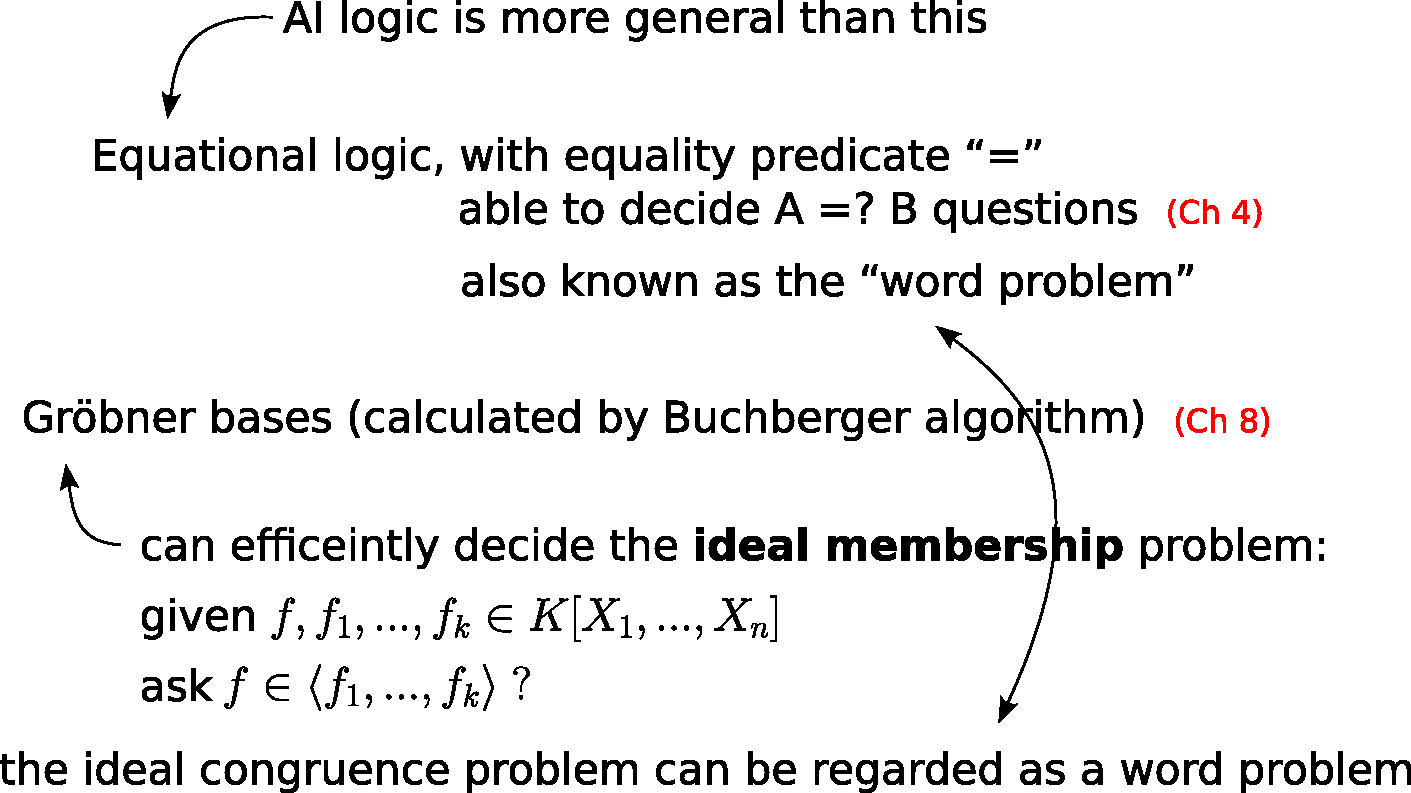
\includegraphics[scale=0.7]{term-rewriting-and-all-that.png}}}
\end{equation}

\begin{itemize}
	\item What is the \textbf{word problem}? \\
	is defined for an equational theory $E$. \\
	is the problem of deciding whether $s = t$
	
	\item why is Gr\"{o}bner basis equivalent to the word problem? \\
	to ask ideal congruence $f =? g$ means $f - g \in? J$ \\
	which is ideal membership problem \\
	a polynomial can be regarded as a rewrite rule \\
	because $f = 0$, we can take the ``largest monomial'' in $f$ as the LHS, and the rest of $f$ as RHS. \\
	In other words:  ideal = set of rules \\
	We ask if a polynomial can be rewritten by the set of rules to another form.  \\
	This is similar to logic deduction.
	
	\item Here an important question is: polynomial reduction seems unable to handle \textbf{logic variables}, it seems only capable of \textbf{simple symbolic rewriting}.
	
	\item logic is equivalent to what form of polynomials? \\
	taking the cue that Huet's higher-order unification = Buchberger algorithm, ...
\end{itemize}

\section{How to study symmetries in deep learning?}

In the following, we will use this sentence as example:
\begin{equation}
	\mbox{\textit{The quick brown fox jumps over the lazy dog}}
\end{equation}
which is a sequence of length $n = 9$.

Matrix formula for Self-Attention:
\begin{align}
	Q &= W^Q X \nonumber \\
	K &= W^K X \nonumber \\
	V &= W^V X \nonumber \\
	\boxed{\mbox{output}} \quad  Z &= \mathrm{softmax} \left( \frac{ Q K^\top }{\sqrt{d_k}} \right) V
	\label{eqn:self-attention}
\end{align}
Take the convention that $X$ consists of ``word vectors'' as \textbf{row} vectors, stacked up to form a matrix of height $n$ which is the sequence length.  The equivariant symmetry says that if we swap any two row vectors in $X$, then the output $Z$ would also have the same rows swapped.  Is this symmetry easy to spot from equation \ref{eqn:self-attention}?  (Note: softmax does not change the structure of its matrix argument, so structurally the output matrix is just $QK^\top V$.)  Perhaps if the reader is very good at linear algebra, but I could not see it.

Figure (\ref{fig:self-attention}) makes it easier to see the matrices' dimensions, but the symmetry is still not apparent.
\begin{figure}
\begin{equation}
\vcenter{\hbox{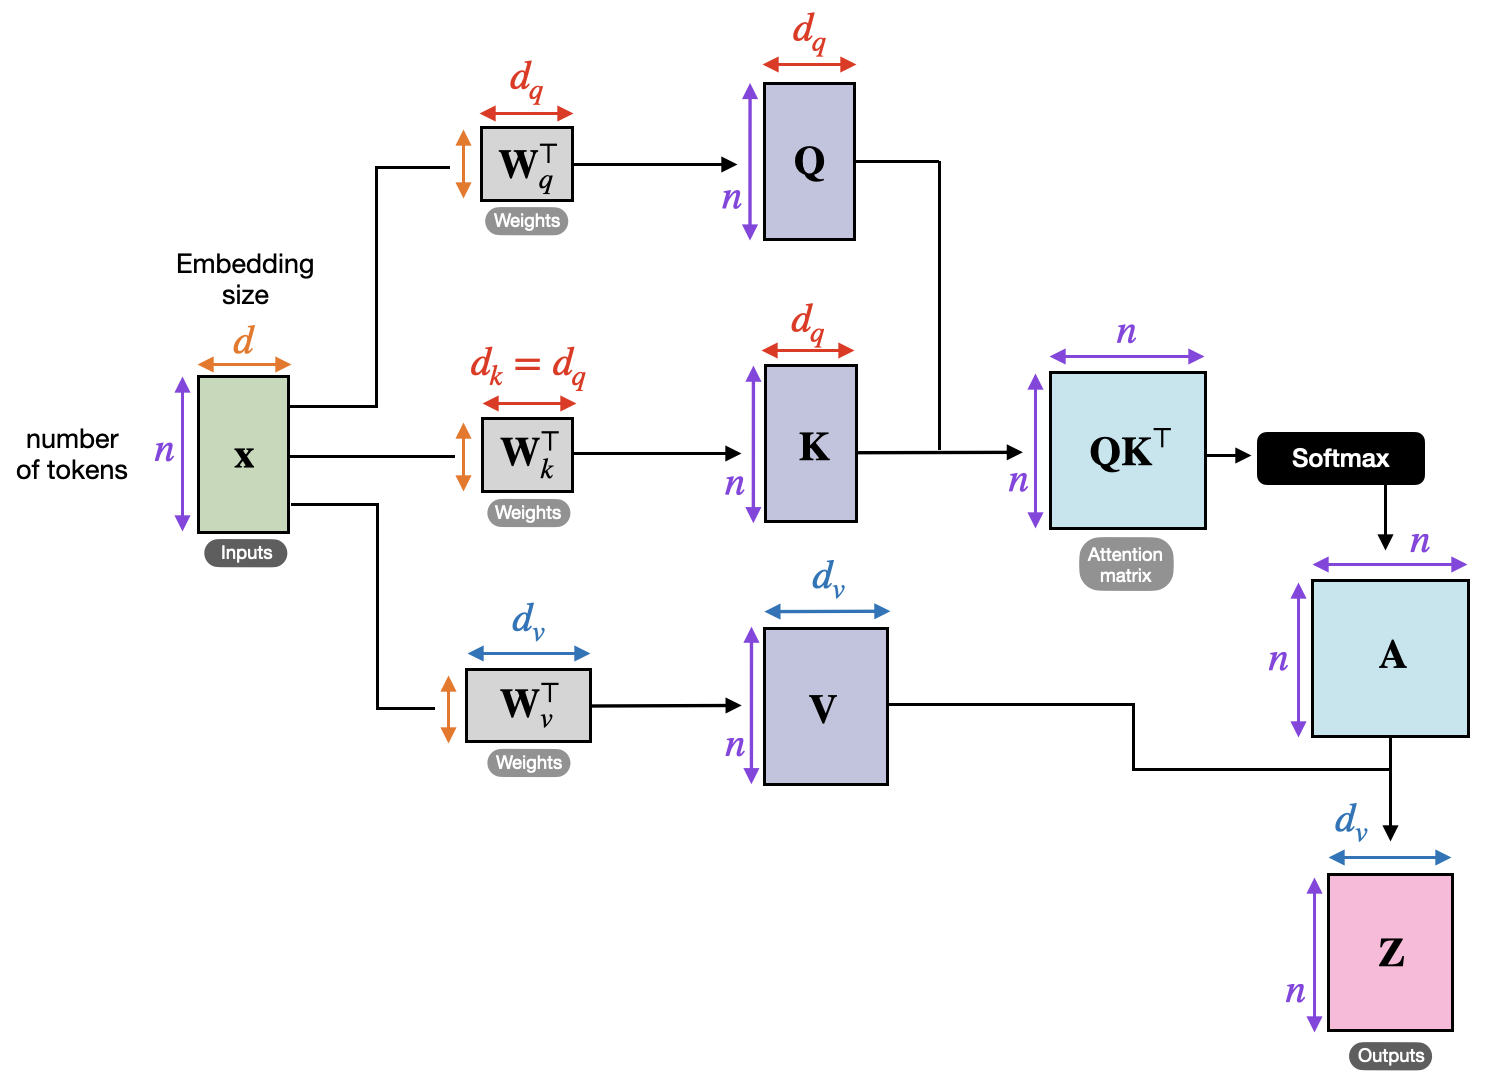
\includegraphics[scale=0.5]{self-Attention.png}}}
\label{fig:self-attention}
\end{equation}
\end{figure}

The way I ``see'' the symmetry can be described verbally as follows:  Imagine \textit{Fox} and \textit{Dog} swapped positions at the input.  The table-lookup operations $W^Q, W^K$ and $W^V$ do not change the rows structure.  When \textit{Fox} is the \textbf{pivot} of its rule, it is matched against Key Key ... Key (which are the same keys as would be matched against \textit{Dog}).  The result for \textit{Fox}'s matching would be a row vector of length $n$, same as for \textit{Dog}.  Since there are $n$ words in the sequence, and each matching involves $n$ keys, the results make up a $n \times n$ matrix, which we call the \textbf{Attention matrix} (after applying softmax, but softmax does not change the structure of the matrix).  In the final matrix multiplication, $[d_V \times n] \times [n \times n] \rightarrow [d_V \times n]$, where one common dimension $n$ on each side has been ``destroyed'' by \textbf{contraction} (dot product).  Another way to say this, not using dot product, is that we have $n$ Value vectors, each Value vector is weighted by one row of the Attention matrix and then added together, resulting in a new Value vector.  This is repeated $n$ times to give $[d_V, n]$.

\begin{figure}
	\begin{equation}
	\hspace{-1.5cm}\vcenter{\hbox{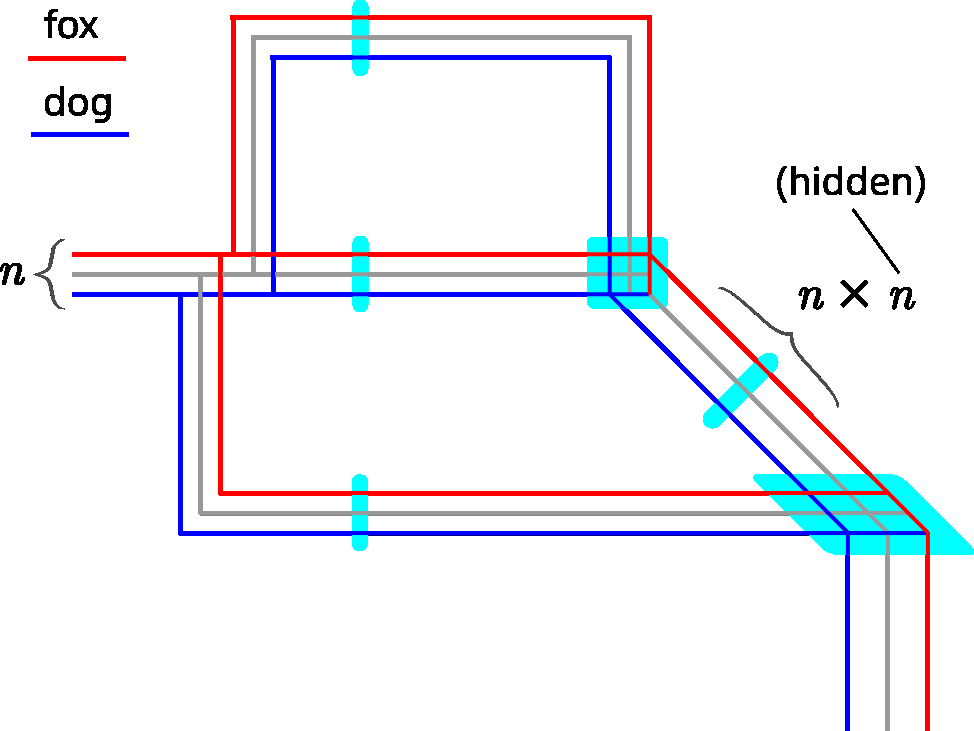
\includegraphics[scale=0.6]{self-attention-string-diagram-2.png}}}
	\qquad
	\vcenter{\hbox{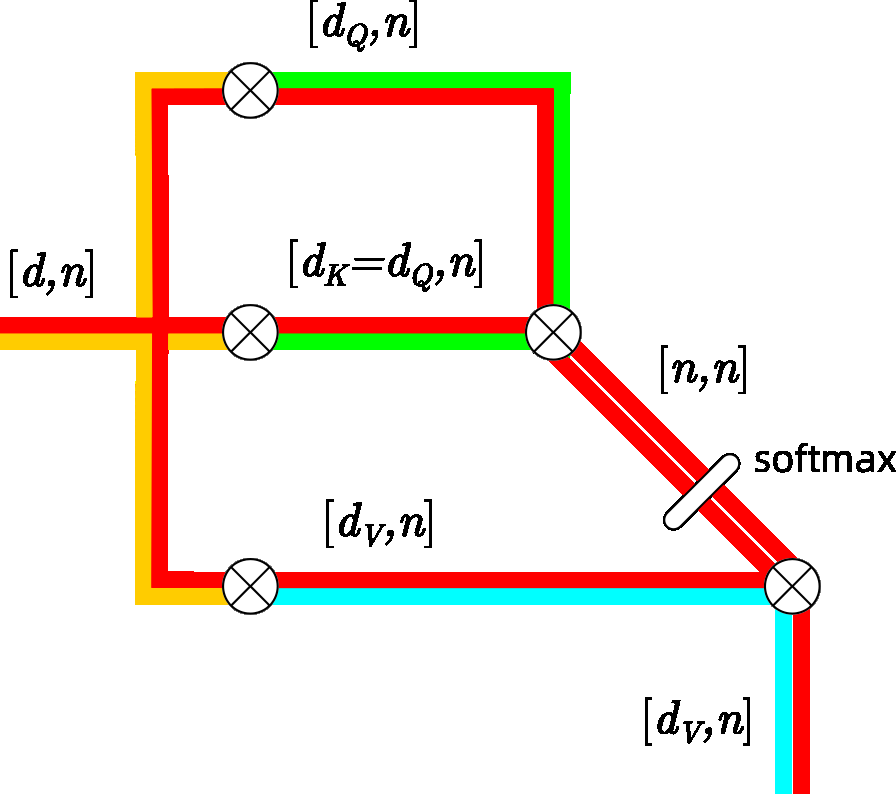
\includegraphics[scale=0.6]{self-attention-string-diagram-3.png}}}
	\label{fig:self-attention-2-and-3}
	\end{equation}
\end{figure}

The simplest example of an equivariance:
\begin{equation}
% method to draw a sigmoid-shape curve:
% \draw (0,0) .. controls (0,4) and (4,0) .. (4,4);
% the controls acts like "magnets"
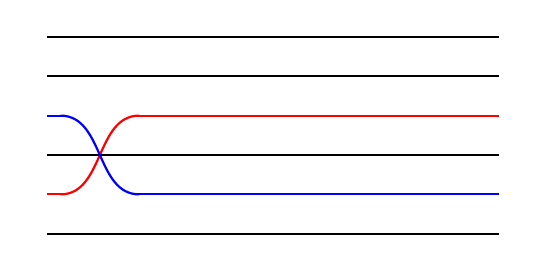
\begin{tikzpicture}[every path/.style={thick}]
\node[] (x0) at (-3, 0) {};
\node[] (x1) at (-3, 0.5) {};
\node[] (1i) at (-2.7, 0.5) {};
\node[] (1j) at (-1.7, 0.5) {};
\node[] (x2) at (-3, 1) {};
\node[] (x3) at (-3, 1.5) {};
\node[] (3i) at (-2.7, 1.5) {};
\node[] (3j) at (-1.7, 1.5) {};
\node[] (x4) at (-3, 2) {};
\node[] (x5) at (-3, 2.5) {};
\node[] (y0) at (3, 0) {};
\node[] (y1) at (3, 0.5) {};
\node[] (y2) at (3, 1) {};
\node[] (y3) at (3, 1.5) {};
\node[] (y4) at (3, 2) {};
\node[] (y5) at (3, 2.5) {};
\draw (x0) to (y0);
\draw[red] (x1) to (1i.center);
    \draw[red] (1i.center) to[out=0,in=-180] (3j.center);
    \draw[red] (3j.center) to (y3);
\draw (x2) to (y2);
\draw[blue] (x3) to (3i.center);
    \draw[blue] (3i.center) to[out=0,in=-180] (1j.center);
    \draw[blue] (1j.center) to (y1);
\draw (x4) to (y4);
\draw (x5) to (y5);
\end{tikzpicture}
\qquad \raisebox{3em}{=} \qquad
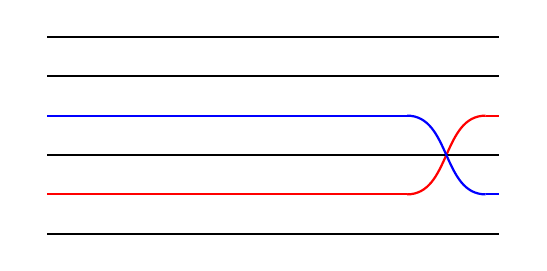
\begin{tikzpicture}[every path/.style={thick}]
\node[] (x0) at (-3, 0) {};
\node[] (x1) at (-3, 0.5) {};
\node[] (1i) at (1.7, 0.5) {};
\node[] (1j) at (2.7, 0.5) {};
\node[] (x2) at (-3, 1) {};
\node[] (x3) at (-3, 1.5) {};
\node[] (3i) at (1.7, 1.5) {};
\node[] (3j) at (2.7, 1.5) {};
\node[] (x4) at (-3, 2) {};
\node[] (x5) at (-3, 2.5) {};
\node[] (y0) at (3, 0) {};
\node[] (y1) at (3, 0.5) {};
\node[] (y2) at (3, 1) {};
\node[] (y3) at (3, 1.5) {};
\node[] (y4) at (3, 2) {};
\node[] (y5) at (3, 2.5) {};
\draw (x0) to (y0);
\draw[red] (x1) to (1i.center);
	\draw[red] (1i.center) to[out=0,in=-180] (3j.center);
	\draw[red] (3j.center) to (y3);
\draw (x2) to (y2);
\draw[blue] (x3) to (3i.center);
	\draw[blue] (3i.center) to[out=0,in=-180] (1j.center);
	\draw[blue] (1j.center) to (y1);
\draw (x4) to (y4);
\draw (x5) to (y5);
\end{tikzpicture}
\end{equation}

Illustration of a function $\vec{f}$ with equivariance property:
\begin{equation}
% method to draw a sigmoid-shape curve:
% \draw (0,0) .. controls (0,4) and (4,0) .. (4,4);
% the controls acts like "magnets"
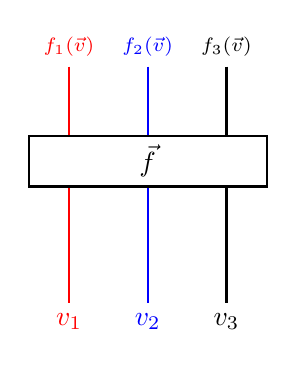
\begin{tikzpicture}[every path/.style={thick}]
\node[red,above] (x0) at (0, 3) {${\scriptstyle f_1(\vec{v})}$};
\node[blue,above] (x1) at (1, 3) {${\scriptstyle f_2(\vec{v})}$};
\node[above] (x2) at (2, 3) {${\scriptstyle f_3(\vec{v})}$};
\node[] (z0) at (0, 1.5) {};
\node[] (z1) at (1, 1.5) {};
\node[] (z2) at (2, 1.5) {};
\node[red,below] (v0) at (0, 0) {$v_1$};
\node[blue,below] (v1) at (1, 0) {$v_2$};
\node[below] (v2) at (2, 0) {$v_3$};
\draw[red] (x0) to (z0.center);
\draw[blue] (x1) to (z1.center);
\draw (x2) to (z2.center);
\draw[red] (z0.center) to (v0);
\draw[blue] (z1.center) to (v1);
\draw (z2.center) to (v2);
\node[inner xsep=40pt,draw,in front of path,fill=white] (f) at (1,1.8) {$\vec{f}$};
\end{tikzpicture}
\qquad \raisebox{5em}{;} \qquad
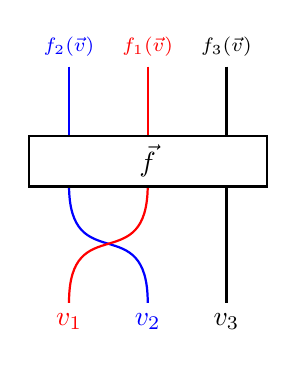
\begin{tikzpicture}[every path/.style={thick}]
\node[blue,above] (x0) at (0, 3) {${\scriptstyle f_2(\vec{v})}$};
\node[red,above] (x1) at (1, 3) {${\scriptstyle f_1(\vec{v})}$};
\node[above] (x2) at (2, 3) {${\scriptstyle f_3(\vec{v})}$};
\node[] (z0) at (0, 1.5) {};
\node[] (z1) at (1, 1.5) {};
\node[] (z2) at (2, 1.5) {};
\node[red,below] (v0) at (0, 0) {$v_1$};
\node[blue,below] (v1) at (1, 0) {$v_2$};
\node[below] (v2) at (2, 0) {$v_3$};
\draw[blue] (x0) to (z0.center);
\draw[red] (x1) to (z1.center);
\draw (x2) to (z2.center);
\draw[blue] (z0.center) .. controls (0,0.3) and (1,1.2) .. (v1);
\draw[red] (z1.center) .. controls (1,0.3) and (0,1.2) .. (v0);
\draw (z2.center) to (v2);
\node[inner xsep=40pt,draw,in front of path,fill=white] (f) at (1,1.8) {$\vec{f}$};
\end{tikzpicture}
\qquad \raisebox{5em}{=} \qquad
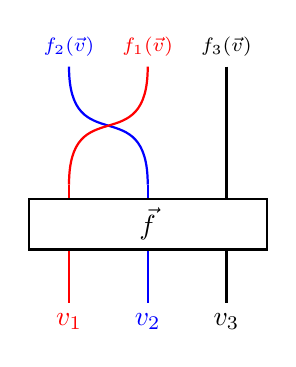
\begin{tikzpicture}[every path/.style={thick}]
\node[blue,above] (x0) at (0, 3) {${\scriptstyle f_2(\vec{v})}$};
\node[red,above] (x1) at (1, 3) {${\scriptstyle f_1(\vec{v})}$};
\node[above] (x2) at (2, 3) {${\scriptstyle f_3(\vec{v})}$};
\node[] (z0) at (0, 1.5) {};
\node[] (z1) at (1, 1.5) {};
\node[] (z2) at (2, 1.5) {};
\node[red,below] (v0) at (0, 0) {$v_1$};
\node[blue,below] (v1) at (1, 0) {$v_2$};
\node[below] (v2) at (2, 0) {$v_3$};
\draw[blue] (x0) .. controls (0,1.8) and (1,2.7) .. (z1.center);
\draw[red] (x1) .. controls (1,1.8) and (0,2.7) .. (z0.center);
\draw (x2) to (z2.center);
\draw[red] (z0.center) to (v0);
\draw[blue] (z1.center) to (v1);
\draw (z2.center) to (v2);
\node[inner xsep=40pt,draw,in front of path,fill=white] (f) at (1,1) {$\vec{f}$};
\end{tikzpicture}
\end{equation}

Practical TO-DO:
\begin{itemize}
	\item implement neural second-order or higher-order logic
	\item enable the creation of random constants (is it useful?)
	\item clarify the role of predicates in HOL, esp its geometric interpretation
\end{itemize}

% 其实想问问就是: 现时理论还能为我们做什么?
% 逻辑 含有「更强」的对称性,但这确切地是什么意思?
% 问题是,暂时我们不太懂得如何量度任意的对称性
% 对称性即「约束」,但此又引申到 参数空间大小的问题
% 如果 参数空间的大小不变,对称性仍可以有强弱之分
% 而以上的观测是严格成立的
% 所以可以说,对称性就是: 在参数空间一样大的情况下,
% 为什么我们说 Attention 比 fully connected 有更强对称性?
% 对称性似乎是相对于 input-output 而言的

The question now is:  what can abstract theory do for us?  We wish to be able to ``compare'' the symmetries possessed by systems.  When doing so, it is important to \textbf{restrict} the number of parameters for all systems in consideration.  This restriction comes from limited computing resource, without which it is meaningless to compare architectures.  After we fixed the number of parameters, two systems, such as fully-connected vs Transformer, could still be different as one possesses equivariant symmetry while the other does not.  This difference in symmetry is what I argue to be crucial to acceleration.

In its most general form an AGI system is defined by the transition function $X_{t+1} = \squareF(X_t)$.  A symmetry can be defined as any group $G$ such that $\squareF$ is invariant or equivariant under its action on the input $X$.  For example, $\squareF(\sigma X) = \sigma \squareF(X), \forall \sigma \in G$.  More generally, any constraint on $\squareF$ could result in acceleration, such as an equation satisfied by $\squareF$.

What is the relation between equivariance of Attention and symmetric NNs of Kolmogorov-Arnold type?

Rewrite neural string diagrams, how?
